\documentclass[sigconf, review, 10pt]{acmart} %timestamp 
%, timestamp
%\usepackage{usenix}
%end of changed lines
\usepackage{microtype}
%\usepackage[hyphens]{url} %Option clash
\usepackage{balance}
\usepackage{leading}
\usepackage{graphicx}
\usepackage{subfig}
%Removing the geometry package used for Tighter Format
%\usepackage{geometry}
%\usepackage{times}
\usepackage{textcomp}
\usepackage{multirow}
\usepackage{framed}
\usepackage{amsmath}
\usepackage{listings}

\usepackage{enumitem}

%\usepackage[usenames,dvipsnames,svgnames,table]{xcolor} %Option Clash
\usepackage[lined,noend,linesnumbered]{algorithm2e}
\usepackage{cleveref}

\crefformat{section}{\S#2#1#3} % see manual of cleveref, section 8.2.1

\newcommand{\sysname}{SciSpot\xspace}

%\newcommand{\comment}[1]{{\color{blue}[\textsf{#1}]}}

%\newcommand{\TODO}[1]{\comment{TODO: #1}}
%\renewcommand{\paragraph}[1]{\textbf{#1}}


\RequirePackage[normalem]{ulem}
\RequirePackage{color}\definecolor{RED}{rgb}{1,0,0}\definecolor{BLUE}{rgb}{0,0,1}
\providecommand{\DIFadd}[1]{{\protect\color{blue}\uwave{#1}}}
\providecommand{\DIFdel}[1]{{\protect\color{red}\sout{#1}}}
%DIF SAFE PREAMBLE
\providecommand{\DIFaddbegin}{}
\providecommand{\DIFaddend}{}
\providecommand{\DIFdelbegin}{}
\providecommand{\DIFdelend}{}
%DIF FLOATSAFE PREAMBLE
\providecommand{\DIFaddFL}[1]{\DIFadd{#1}}
\providecommand{\DIFdelFL}[1]{\DIFdel{#1}}
\providecommand{\DIFaddbeginFL}{}
\providecommand{\DIFaddendFL}{}
\providecommand{\DIFdelbeginFL}{}
\providecommand{\DIFdelendFL}{}
%DIF END PREAMBLE EXTENSION ADDED BY LATEXDIFF

\def\Section {\S}

\newcommand{\squishlist}{
 \begin{list}{$\bullet$}
  { \setlength{\itemsep}{0pt}
     \setlength{\parsep}{3pt}
     \setlength{\topsep}{3pt}
     \setlength{\partopsep}{0pt}
     \setlength{\leftmargin}{1.5em}
     \setlength{\labelwidth}{1em}
     \setlength{\labelsep}{0.5em} } }
	
\newcommand{\squishlisttwo}{
 \begin{list}{$\bullet$}
  { \setlength{\itemsep}{0pt}
     \setlength{\parsep}{0pt}
    \setlength{\topsep}{0pt}
    \setlength{\partopsep}{0pt}
    \setlength{\leftmargin}{2em}
    \setlength{\labelwidth}{1.5em}
    \setlength{\labelsep}{0.5em} } }

\newcommand{\squishend}{
  \end{list}  }

\newcommand{\alert}[1] {\textcolor{red} {\textsc{#1}}}

\newcommand{\myfbox}[1] {\noindent \fbox{\parbox{0.5\textwidth} {#1}}}

\newcommand{\mhead}[1] {\noindent \textbf{#1}}

\newcommand*\mean[1]{\overline{#1}}

\newcommand{\eat}[1]{}

\newcommand{\compresslist}{%
  \setlength{\itemsep}{1pt}%
  \setlength{\leftmargin}{1.5em}
  \setlength{\labelwidth}{1em}
  \setlength{\parskip}{0pt}%
  \setlength{\parsep}{0pt}%
%  \setlength{\itemindent}{-10pt}%
}

\newcommand{\myfigspace}[0]{-0.45cm}
\newcommand{\bigfigspace}[0]{-0.9cm}
\newcommand{\captionspace}[0]{-0.5cm}
\newcommand{\subsecspace}[0]{-0.33cm}
\newcommand{\largesubsecspace}[0]{-0.40cm}
\newcommand{\tightext}[0]{-0.12cm}
\newcommand{\eqnspace}[0]{-0.1cm}

%%% Local Variables:
%%% mode: latex
%%% TeX-master: "paper"
%%% End:


\newcommand{\sign}[1]{\operatorname{sign}\left({#1}\right)}


\newcommand\prat[1]{\textcolor{red}{(Prateek: #1)}}
\newcommand\vikram[1]{\textcolor{green}{(Vikram: #1)}}


%%%%%%%% For submission only

\setcopyright{none}
\settopmatter{printacmref=false}
\acmConference{}{}{}
\acmPrice{}
\acmISBN{}
\acmDOI{}
\acmYear{}
\acmMonth{}
\settopmatter{printfolios=true}
%%%%%%%%%%%%%%%%%%%


\begin{document}
\title{SciSpot}
\author{Paper \# XXX}{}{}

\begin{abstract}
  In this paper, we...
%%% Local Variables:
%%% mode: latex
%%% TeX-master: "paper"
%%% End:

\end{abstract}

\maketitle

\section{Introduction}

Running parallel scientific applications, such as molecular dynamics (MD) simulations, on low-cost cloud transient resources. 

The first "big" idea is that simulations are often bag of parallel tasks. 

While there has been some past work that looks at running MPI applications on spot instances, our scope is much broader and considers how complete simulation pipelines can be run at low cost. 

Spiel on transient instances. Increasingly popular resource allocation model that is being offered by all cloud providers. 
Very low cost compared to conventional cloud resources, often by up to 10x. 
However, can be frequently revoked. 
Thus failure is a common occurrence, and not a rare-event. 
This is especially challenging for MPI jobs because of its inability to tolerate failures. 

However, our insight is that while protecting a *single* job against revocations can require elaborate checkpointing based approaches, we dont necessarily have to do that if we consider that most simulations are composed of a series of jobs that search over a parameter space, and that what is important is the total running time and cost of this entire series of jobs. 

Thus, no single job is "special". 

Another aspect of novelty is that past work on transient resources used EC2 pricing information to get failure probabilities. However, this is no longer an accurate method. We perform the first empirical study of google preemptible VMs and their performance and availability for HPC workloads. 

Another fundamental question is what is a suitable metric in such cases. Conventionally, it is speedup. In the cloud, it is some combination of cost and running time. 

%%% Local Variables:
%%% mode: latex
%%% TeX-master: "paper"
%%% End:


\sysname is a framework and a tool that combines the use of failure modeling, checkpointing, and application-aware early stopping, to provide low cost execution of jobgroups for scientific applications.


Our work is the first to make a principled study of transient instances \emph{other} than Amazon spot instances.
Furthermore, our techniques make the first stab at addressing the new problems in the new EC2 spot pricing scheme.





\section{Background}

\subsection{Transient Computing}

%\subsection{Heterogeneity and Parallel Scientific Applications in the Cloud}

%No extra parallelism required
%RM heterogen

%
\subsection{Case Studies: Bags of Jobs in Scientific Computing Applications}

\begin{comment}
Describe the kind of computation. DONE

Scaling properties. Almost perfectly scalable with O(n) communication? UNCLEAR WHAT IS MEANT TO BE DONE HERE

This can be a like a case study of parallel scientific simulations.
Will help relate to parameters etc with more concrete examples. DONE

Bag of jobs.
Why multiple runs: parameter sweeps, search, or just multiple times to get confidence intervals and stable results in case of randomness. 
DONE I THINK
\end{comment}

For testing and evaluating the SciSpot framework, we consider three representative examples (case studies) from molecular dynamics (MD) and hydrodynamics simulations: 1) MD simulations of ions in nanoscale confinement created by material surfaces \cite{jjzo1,kadupitiya2017}, MD-based optimization dynamics of shape-changing deformable nanoparticles (NPs) \cite{jto1,jyto}, and hydrodynamics simulations of continuum material models using the Livermore Unstructured Lagrangian Explicit Shock Hydrodynamics (LULESH) code \cite{IPDPS13:LULESH,LULESH2:changes}. These examples are representative of typical scientific computing applications in the broad domain of physics, materials science, and chemical engineering; the first two applications (1 and 2) are based on codes and associated theoretical formulations developed by us \cite{jso1,jso2,solis2013generating,jjzo1,jto1,jyto}, and case study 3 is based on an open-source code developed at Lawrence Livermore National Laboratories \cite{IPDPS13:LULESH,LULESH:spec}. These three examples are implemented as parallel programs that use OpenMP and MPI parallel computing techniques.

The typical workflow associated with most scientific computing applications, including the aforementioned case studies, involves the implementation of the ``bags of jobs'' approach at many critical stages. In the initial stage, the construction and calibration of the appropriate model often involves testing for the needed attributes (e.g., characteristic sizes, interactions potentials) of the building blocks (model components) by sweeping over different combinations of physical as well as computing parameters (e.g., simulation timestep, thermostat variables) and eliminating the sets that lead to unphysical, unstable, or computationally intractable scenarios. During the model examination stage for the investigation of the accuracy and generalization of the model to describe the associated natural or synthetic processes, the dynamics of the model system is simulated over a wide range of model parameters. Accordingly, multiple sets of simulations (bags of jobs) are run to sweep over a broad region of the multidimensional parameter space and to isolate the domains where the model works best and where it yields a poorer representation of the real system. 

Often, the key objective of the scientific computing application is to isolate the model system parameters where interesting changes in the material structure or assembly behaviors (e.g., phase transitions) are observed. A similar bags of jobs approach is also  adopted in such applications with the search for these model parameters generally inspired by experimentally-informed observations and/or predictions yielding from approximate analytical theoretical formulations. For example, in the simulation of deformable nanoparticles implemented in the NP shape code, one is interested in isolating the set of NP and environmental parameters: NP bending modulus, NP stretching constant, NP charge, and salt concentration, that yields complex NP deformations/shapes (e.g., discs, rods, bowls). Similarly, in the ions in nanoconfinement application, a quantity of interest is the set of electrolyte system attributes (parameters): confinement length $h$, positive ion valency ($z_p$), negative ion valency ($z_n$), electrolyte concentration $c$, and ion diameter $d$, that yields the expected contact density or the experimentally-measured effective pressure between the confining nanomaterial surfaces. Finally, the bags of jobs approach is adopted during the completion process in the workflow where simulations are often launched in parallel to fill any gaps in the extracted trends or to obtain error bars on the predictions (e.g., ionic density profiles, energy distributions, NP shape transitions).

In addition to the conventional scientific computing (HPC) applications, an emerging area of research in a broad range of fields including materials science, biology, neuroscience, and physics where the bags of jobs approach is critical to the workflow is the integration of machine learning (ML) tools with these HPC applications  \citep{ml.atomic2017,melko2017,sam2017,fu2017,long2015machine, ferguson2017machine,ward2018matminer,jcs1,jcs2,fox2019learning}. ML methods have been developed and implemented to identify model attributes/parameters that yield desirable material configurations \citep{glotzer2017}, update configurations in simulations \citep{botu2015adaptive,fu2017}, predict and auto-tune optimal simulation control parameters \cite{jcs1}, predict critical features associated with simulation output \cite{jcs2}, infer assembly landscapes \citep{long2015machine,ferguson2017machine}, and classify phases of matter \citep{melko2017}. In many of these examples, ML models (e.g., artificial neural network, support vector machines) are trained on large data sets generated via simulations run over a broad range of parameter values. The bags of jobs process is invoked multiple times during the experimentation with many ML techniques using training and testing datasets to isolate the ML method(s) that yield the most accurate results for a given scientific computing application. For example, in Ref.~\cite{jcs2}, an ANN was trained to predict contact, peak, and mid-point ionic density using training and testing datasets comprising of $\approx4800$ and $\approx2000$ simulation runs respectively. Datasets were generated using HPC resources (Bigred2 computing cluster) based on the sweep of parameters $h \in (3.0, 4.0)$ nm,  $z_p \in 1,2,3$ (in units of electronic charge $|e|$); $z_n \in -1,-2$ $|e|$; $c \in (0.3,0.9)$ M, and $d \in (0.5,0.75)$ nm. We envision the SciSpot framework described here to complement and supplement conventional HPC supercomputer systems in enabling the construction of such ML layers (wrappers) \cite{jcs2,fox2019learning} around scientific computing applications. 

%%% Local Variables:
%%% mode: latex
%%% TeX-master: "paper"
%%% End:


\section{Design}

Scientific simulation applications consume a large amount of computational resources, and are often used in the context of \emph{exploratory} research, where a large amount of jobs are run with  different simulation parameters.
This can be either a \emph{parameter sweep}, where a large number of parameters need to be evaluated, or a \emph{search} over a large parameter space for the ``right'' set of parameters that yield the desired model behavior.

In this paper, we look at the problem of running scientific simulations on \emph{transient} computing resources in public clouds. 


Past work has largely been focused on running parallel jobs (such as MPI) in the cloud. 
However, considering entire \emph{job-groups} or ensembles of jobs presents new challenges and opportunities in timely, low-cost computation.

Our system, \sysname, is a unified framework for running large job-groups that result from parameter exploration. 

Input and some assumptions:
We assume that the job-group consists of $J_1\ldots J_N$, with each job evaluating a model on some parameter.
The list of parameters to explore can either be generated apriori (as in the case of parameter sweeps), or be dynamically generated as in the case of a search.

In this section, we will look at how we address these challenges:
\begin{enumerate}
\item How to select the right type of cloud server for an application?
\item How to effectively run job-groups?
\end{enumerate}

\sysname's key insight is considering an entire job-group can allow better and simpler optimizations that can be easily deployed. 



\subsection{Trade-offs in Server Selection}

This presents us with many challenges in the cloud-deployment of these jobs.

Cloud providers offer multiple types of instances (VMs), with different hardware configuration (such as number of CPUs and memory size).
The price of cloud servers is related to their hardware configuration, but it may not be strictly proportional to the hardware performance.
For example, a VM with 32 CPUs may not be 32 times the cost of a single CPU VM.


For parallel and distributed applications, the type of servers selected has large implications on their performance.
Consider the case of deploying an application on 8 8-core VMs vs. 16 4-core VMs.
In both cases, the total number of CPU cores is the same.
However, the larger number of VMs requires more communication between the application tasks, and thus may result in performance degradation.
The performance of applications at different cluster configurations depends on their communication patterns and scaling properties. 



Thus, when deploying applications on the cloud, one has to mindful of the cost and performance tradeoff.
However, in the case of transient servers, the story does not stop here. 


In addition to pricing differences, the transient availability of instances \emph{also} differs by type.
Because the availability of a transient VM is broadly determined by the overall supply and demand of the instances of that \emph{particular} type, the ``preemption rate'' of VMs often depends on the type of the instance.



Thus, selecting a transient cloud server involves a complex tradeoff between the cost of servers, their performance, and the preemption-rate.


\subsection{Server Selection Policy}

\sysname's server selection policy seeks to identify the best server type for a given job-group.

As stated in the previous subsection, the transient server selection problem is challenging because it involves balancing multiple optimization criteria: applications want low cost, low preemptions, and high performance.

Server selection based on application characteristics is a subject of a growing amount of recent work.
These approaches often use micro benchmarks to gather performance data of cloud servers, and then use application performance models to determine suitable VMs for a specific application.
Another class of approaches uses ``black box'' performance modeling, where the application's performance is modeled using a function of the resources, for example, by using linear regression.

In contrast to prior work, our server selection employs a ``cold start'' policy, and we do not run profiling or pilot jobs that can increase the overall running time and cost.
Instead, we search for the ``best'' cluster configuration for jobs in a job-group, by exploring the cluster configuration space for the ``optimum'' server type that optimizes all the desired parameters: cost, running time, and revocation rate.


Thus, the first $e$ jobs in the job group $J_1\ldots J_e$ are the exploration jobs, run on different cluster configurations.
We limit the total number of combinations to explore, by allowing users to submit an estimate of the total number of CPU cores that they desire for each job.
This allows us to meet the user expectations in terms of performance and cost---whether the user expects us to spend a large amount of resources or not.

Thus, assuming that there are $s$ different types of VM instances, the first $s$ jobs are run on the $s$ different types.
Note that we use homogeneous clusters, since the performance of BSP programs in Heterogeneous environments can be degraded, and importantly, as we show, there are no performance or cost benefits to Heterogenity. 


For each server type $i$, we calcuate the expected cost $E[C_i]$.

$E[C_i] = n_i*c_i * E[T_i]$, where $c_i$ is the price (per second) of the server, $n_i$ is the number of servers of that type required to meet the core-count requirement.
The expected running time of the job depends on two factors: the actual running time $T$, and the increase in running time due to preemptions.
Each preemption is akin to a fail-stop failure, which requires an application to restart.
Our system makes no assumptions about the fault-tolerance policies supported by the application. For example, some applications may be able to \emph{checkpoint} their state periodically.
In either case (checkpointing or not), there is some work lost due to revocations.
For ease of exposition, we assume no checkpointing. We discuss checkpointing in the next section (or never?)


\mhead{Expected running time:}
Let the running time without failure be T:

\begin{equation}
  \label{eq:et1}
E[T_i] = T + P(\text{at least one failure})*T/2   
\end{equation}

For calcuating the probability of failure, we assume that the failure rate of an individual server of the type is $p_i$. 

\begin{align}
  \label{eq:pfail1}
  P(\text{at least one failure}) &= 1-P(\text{no failure}) \\
                                 &= 1-(1-p_i)^{n_i} 
\end{align}

Thus, we can see that if we select smaller VMs, we will require more of them (higher $n_i$), and this cluster configuration will have a larger probability of failure and thus higher running times and costs.

The probability of failure $p_i$ depends on the type of server, and we use historically determined failure distributions.
Roughly, if we assume exponentially distributed failures, then:
\begin{equation}
  \label{eq:pi}
  p_i = \dfrac{T}{\text{MTTF}_i}
\end{equation}

Where MTTF is the mean time to failure of the server type, and T is the empirically determined job running time without failures (the best case).






In addition to searching over the servers, the effective number of servers is also dynamic in the case of transient environments due to preemptions.
Thus, once we have found the appropriate server, we then explore the application's performance at smaller cluster sizes, which helps in the job-group policies that we discuss next. 


\subsection{Preemption-handling Policies}

We run the remaining jobs on the right configuration that is determined through the server selection policy.

Our goal is to minimize costs given a deadline.

This determines two things: how many jobs should be run in parallel, and what to do upon a revocation.

The number of jobs in parallel determines the overall size of our cluster.

$\text{number of parallel jobs} = \dfrac{N\cdot T}{\text{Deadline Duration}}$

If a server is preempted, then the job running on it will cease to run.
Our preemption handling policies then decide what to do:
\begin{enumerate}
\item Restart the job on a smaller number of servers 
\item Replenish lost servers and restart job
\item Discard job. This may be useful in case of parameter sweeps. 
\end{enumerate}

In addition, the user is also allowed to provide the fraction of jobs that are allowed to fail ($\eta$).


\subsection{Checkpointing}

Checkpointing requires the same number of servers, which may be tricky, whereas restarts can be on smaller number of nodes no problem.


\subsection{Early Stopping}

Based on the energy function, we can stop some simulations early.
The early stopping criteria helps in minimizing the number of jobs run to completion.

We use this to proactively monitor jobs, as well as to decide whether to restart a job if it is preempted.

*This can be a fairly substantial section*



%%% Local Variables:
%%% mode: latex
%%% TeX-master: "paper"
%%% End:


%\vspace*{\subsecspace}
%\section{SciSpot Design and Implementation}
\subsection{Details of the Experimental Framework used for Evaluation}
%\section{Model-Informed Policy Implementation}
\label{sec:impl}


\sysname is a general-purpose software framework for running scientific computing applications on low-cost transient cloud servers.
It incorporates policies and mechanisms for generating, deploying, orchestrating, and monitoring bags of jobs on cloud servers.
Specifically, it runs a bag of jobs defined by these parameters:
\begin{lstlisting}[basicstyle=\sffamily, frame=single, columns=fullflexible, escapeinside={(*}{*)}]
  Bag of job = {(*$\mathcal{A}$*): Application to execute,
  (*$n$*): Number of jobs,
  (*$m$*): Minimum number of jobs to finish,
  (*$\pi$*): Generator function for job parameters,
  (*$\mathcal{R}$*): Computing resources per job}
\end{lstlisting}


%Additionally, ease-of-use is one of \sysname's primary design goals, and we specifically incorporate

%it is suitable for running a large variety of applications.
\sysname seeks to minimize the cost and running time of bags of jobs of scientific computing applications.
\sysname's cost and time minimizing policies for running bags of jobs are based on empirical and analytical models of the cost and preemption dynamics of  transient cloud servers, which we present in the next section. 

\sysname is designed as a framework that increases the usability and viability of transient cloud servers for scientific computing applications, and provides a simple user interface to allow users to deploy their applications with minimum workflow changes. 
Most scientific computing applications are deployed on HPC clusters that have a batch scheduler such as Slurm~\cite{slurm} or Torque~\cite{torque}, and \sysname integrates with these schedulers (e.g., Slurm) to provide the same interface to applications. 
As shown in Figure~\ref{fig:arch},
\sysname creates and manages clusters of transient cloud servers, manages all aspects of the VM lifecycle and costs, and implements the various policies described in the rest of this section. 

\begin{figure}[t]
  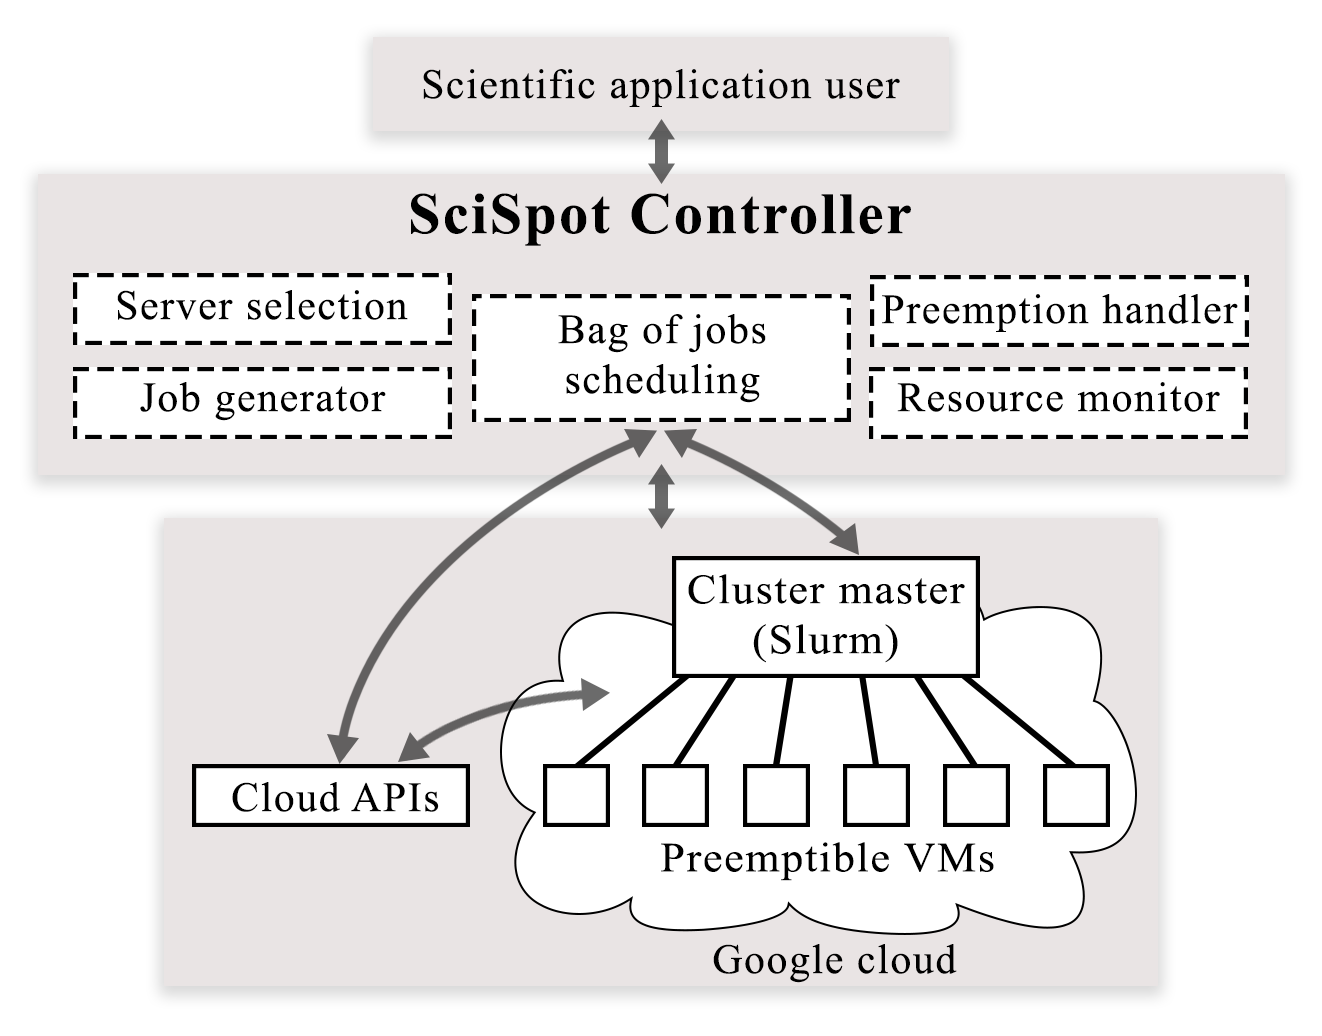
\includegraphics[width=0.3\textwidth]{../figures/Architecture.png}
\vspace*{\myfigspace}
  \caption{SciSpot architecture and system components.}
  \label{fig:arch}
  \vspace*{\myfigspace}
\end{figure}


\noindent \textbf{High-level workflow:} When a user wishes to run a bag of jobs, \sysname handles the provisioning of a cluster of transient cloud servers.
In addition, \sysname deals with the scheduling and monitoring of the bag of jobs, and with VM preemptions. 
Execution of a bag of jobs proceeds in two phases.
In the first phase, \sysname selects the ``right'' cluster configuration for a given application through a cost-minimizing exploration-based search policy, described in Section~\ref{subsec:server-selection}. 
In the second phase, \sysname proceeds to run the remaining jobs in the bag on the optimal cluster configuration. 

\prat{End design}


\sysname is implemented as a light-weight, extensible framework that makes it convenient and cheap to run scientific computing applications in the cloud.
We have implemented the \sysname prototype in Python in about 2,000 lines of code, and currently support running VMs on the Google Cloud Platform~\cite{gcp}. 
%
\sysname is implemented as a centralized controller, which implements the VM selection and job scheduling policies described in Section~\ref{sec:design}. 
The controller can run on any machine (including the user's local machine, or inside a cloud VM), and exposes an HTTP API to end-users. 
Users submit bags of jobs to the controller via the HTTP API, which then launches and maintains a cluster of cloud VMs, and maintains the job queue and metadata in a local database. 
To improve usability, we automatically generate parameter combinations for a given bag size, based on a user-provided json file with ranges and constraints for each parameter. 

\sysname integrates, and interfaces with two primary services.
First, it uses the Google cloud API~\cite{gcloud-api} for launching, terminating, and monitoring VMs.
Once a cluster is launched, it then configures a cluster manager such as Slurm~\cite{slurm} or Torque~\cite{torque}, to which it submits jobs. 
\sysname uses the Slurm cluster manager, with each VM acting as a Slurm ``cloud'' node, which allows Slurm to gracefully handle VM preemptions.
The Slurm master node runs on a small, 2 CPU non-preemptible VM, which is shared by all applications and users. 
\sysname monitors job completions and failures (due to VM preemptions) through the use of Slurm call-backs, which issue HTTP requests back to the \sysname controller.

%As part of \sysname, we also provide a base VM image with Slurm and MPI integration, along with commonly used libraries and benchmarks for scientific computing. To run an application, users must provide a location to the application source code or binaries. Integrating \sysname with container-based image management tools such as Docker~\cite{docker} and Singularity~\cite{kurtzer2017singularity} is part of our ongoing work. 





%%% Local Variables:
%%% mode: latex
%%% TeX-master: "paper"
%%% End:


\vspace*{\subsecspace}
\section{Experimental Evaluation}
\label{sec:eval}

%Opening is deliberately short because we gonna be running out of space 
In this section, we present empirical and analytical evaluation of the performance and cost of \sysname under different workloads and scales. 
Our evaluation consists of empirical analysis of the different scientific computing applications, as well as model-driven simulations for analyzing and comparing \sysname behavior under different preemption and application dynamics. 

% \begin{itemize}
% \item What is performance and cost of 
% \end{itemize}

\noindent \textbf{Environment and Workloads:} All our empirical evaluation is conducted on the Google Public Cloud, and with these representative scientific computing applications: 
% open-source
%\vspace*{\tightext}
%\begin{description}
  %TODO: Need MAX two sentence descriptions

\noindent \textbf{Nanoconfinement.}
The nanoconfiment application launches molecular dynamics (MD) simulations of ions in nanoscale confinement created by material surfaces \cite{jyto,kadupitiya2017}.

\noindent \textbf{Shapes.} The Shapes application runs an MD-based optimization dynamics to predict the optimal shape of deformable, charged nanoparticles \cite{jto1,jjzo1}. 

\noindent \textbf{LULESH.} Livermore Unstructured Lagrangian Explicit Shock Hydrodynamics (LULESH) code is a popular code to for hydrodynamics simulations of continuum material models \cite{IPDPS13:LULESH,LULESH2:changes}. 
%\end{description}
%\vspace*{\tightext}

These examples are representative of typical scientific computing applications in the broad domain of physics, materials science, and chemical engineering. These three examples are implemented as parallel programs that use OpenMP and MPI parallel computing techniques. The first two are used in nanoscale materials research \cite{jso1,jso2,solis2013generating,jjzo1,jto1,jyto} and the LULESH is a widely used benchmark \cite{IPDPS13:LULESH,LULESH2:changes}. All applications are run with default parameters unless otherwise stated. 
All applications use OpenMPI, are deployed on Slurm vXXX and 64-bit Ubuntu 18.04, and run on Google Cloud VMs with x86-64 Intel Broadwell CPUs. 
%Networking? 


\vspace*{\subsecspace}
\subsection{SciSpot Performance and Cost}

%%%%%%%%%%%%%%%%%%%%%%%%%%%%%%%%%%%%%%%%%%%%%%%%%%
\subsubsection{Impact of server exploration}

As described in Section~\ref{sec:design}, applications can be deployed on multiple types of VMs in the cloud, with each VM type having a different ``size''.
In our evaluation of parallel scientific computing applications that are CPU intensive, we are primarily interested in the number of CPUs in a VM.

When an application (i.e., bag of jobs) requests a total number of CPUs to run each of its jobs, \sysname first runs its exploration phase to find the ``right'' VM for the application.
\sysname searches for the VM that minimizes the total expected cost $E[C_{(i,n_i)}]$ of running the application, and this depends on several factors such as the parallel structure of the application, the preemption probability and the associated job recomputation time, and the price of the VM.

Thus, even if the \emph{total} amount of resources (i.e., number of CPUs) per job is held constant, the total running time of an application depends on the choice of the VM type ($i$), and the associated number of VMs ($n_i$) required to meet the allocation constraint (Section~\ref{subsec:cost-model}).
%
With preemptible instances, the total running time of a job is composed of two factors: the ``base'' running time of the job without any preemptions ($T_{(i,n_i)}$), and the expected recomputation time which depends on the probability of job failure (Equation~\ref{eq:et1}). 

\begin{figure}
  \centering
  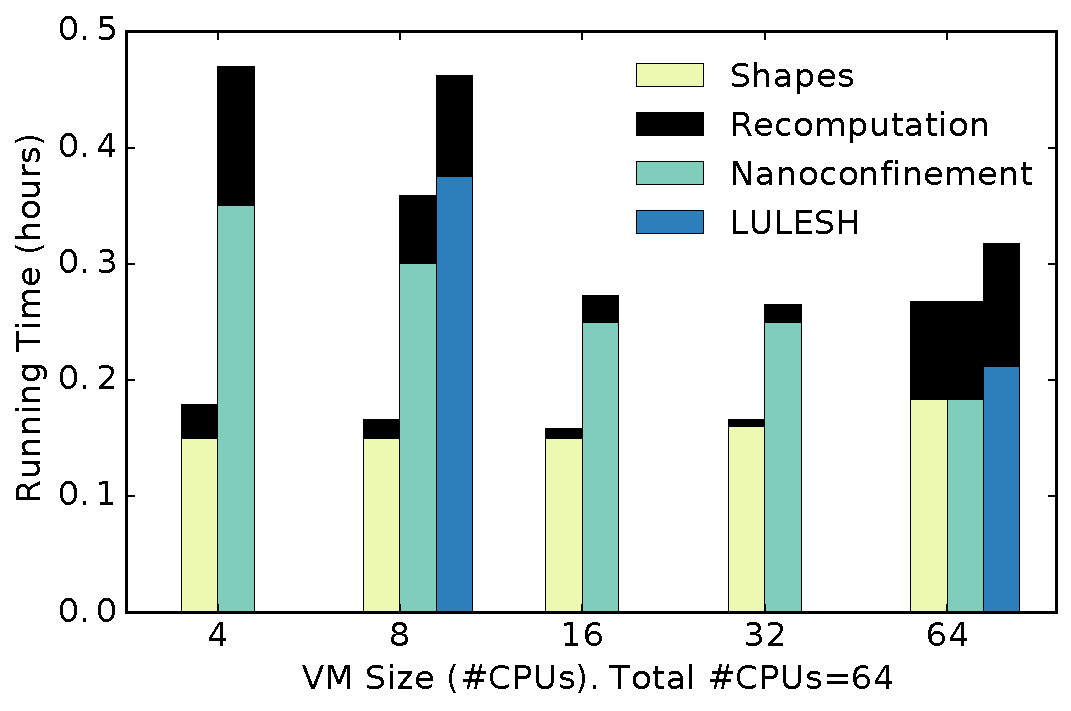
\includegraphics[width=0.4\textwidth]{../graphs/runtime-bars.pdf}
      \vspace*{\myfigspace}
  \caption{Running times of applications on different VMs. The total number of CPUs is 64, yielding different number of VMs in each case. We see different tradeoffs in the base running times and recomputation costs for the different applications.}
  \label{fig:runtimes-bar}
    \vspace*{\myfigspace}
\end{figure}


Figure~\ref{fig:runtimes-bar} shows the running times of the Nanoconfinement and Shapes application, when they are deployed on different VM sizes.
In all cases, the total number of CPUs per job is set to 64, and thus the different VM sizes yield different cluster sizes (e.g., 16 VMs with 4 CPUs or 32 VMs with 2 CPUs).


For the Nanoconfinement application, we observe that the base running times (without preemptions) reduce when moving to larger VMs, because this entails lower communication costs.
The running time on the ``best'' VM (i.e., with 32 CPUs) is nearly 40\% lower as compared to the worst case. 
On the other hand, the Shapes application can scale to a larger number of VMs without any significant communication overheads, and does not see any significant change in its running time.

Figure~\ref{fig:runtimes-bar} also shows the total expected running time $E[T_{(i,n_i)}]$, that is obtained by adding the the expected recomputation time, which depends on the expected lifetimes of the VM and the number of VMs, and is computed using the cost model introduced in Section~\ref{subsec:cost-model}. 
While selecting larger VMs may reduce communication overheads and thus improve performance, it is not an adequate policy in the case of preemptible VMs, since the preemptions can significantly increase the total running time.
We can observe this in the case of Nanoconfinement application when deployed on a 64 CPU VM---even though the base running time is lower compared to deploying the application on 2x32-CPU VMs, the recomputation time on the 64 CPU VM is almost $4\times$ higher due to the much lower expected lifetime of the larger VMs. 
Thus, on preemptible servers, there is a tradeoff between the base running time which only considers parallelization overheads, and the recomputation time.
By considering \emph{both} these factors, \sysname's server selection policy can select the best VM for an application. 


\noindent \emph{\textbf{Result:} SciSpot's server selection, by considering both the base running time and recomputation time, can improve performance by up to 40\% , and can keep the increase in running time due to recomputation to less than 5\%.}

%%%%%%%%%%%%%%%%%%%%%%%%%%%%%%%%%%%%%%%%%%%%%%%%%%
\subsubsection{Cost}

\begin{figure}
  \centering
  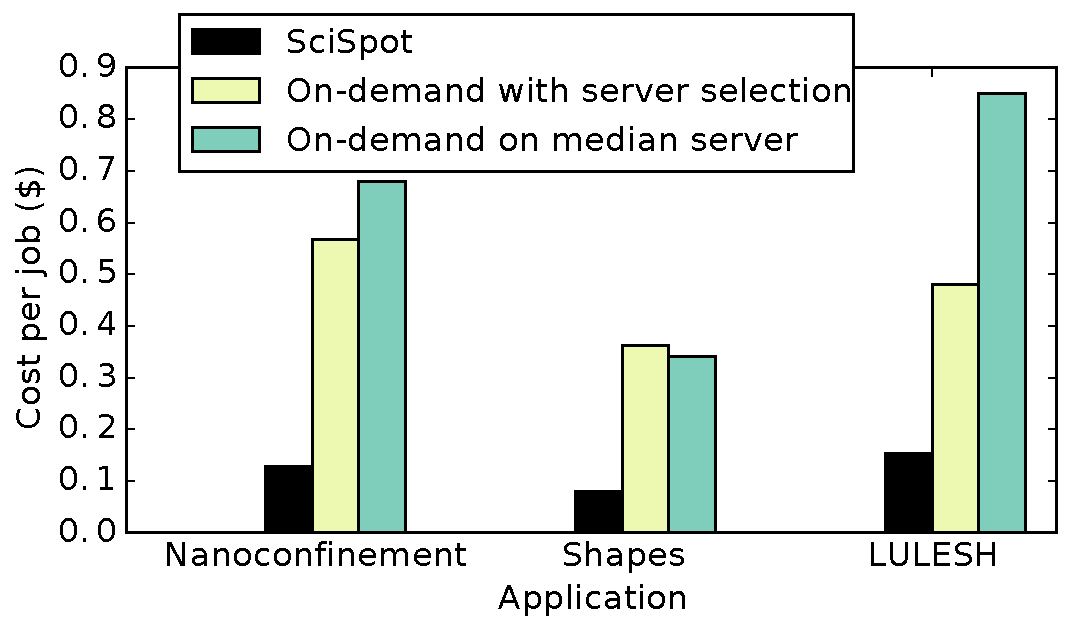
\includegraphics[width=0.4\textwidth]{../graphs/cost-only-bar.pdf}
  \vspace*{\myfigspace}
  \caption{SciSpot's use of preemptible VMs can reduce costs by up to $5\times$ compared to conventional cloud deployments.}
  \label{fig:cost-only-bar}
    \vspace*{\myfigspace}
\end{figure}


The primary motivation for using preemptible VMs is their significantly lower cost compared to conventional ``on-demand'' cloud VMs that are non-preemptible. 
Figure~\ref{fig:cost-only-bar} compares the cost of running different applications with different cloud VM deployments.
\sysname, which uses both cost-minimizing server selection, and preemptible VMs, results in significantly lower costs across the board, even when accounting for preemptions and recomputations. 
Even with \sysname's server selection, using on-demand VMs result in a $5\times$ cost increase compared to \sysname.
In the absence of server selection, we assume that the user will pick a ``median'' VM in terms of number of CPUs (in this case, 8 CPU VMs), which we also show in Figure~\ref{fig:cost-only-bar}.
Note that since \sysname's server selection considers the total turnaround time (which includes recomputation time), it may not always pick the optimal on-demand server. 

%\vj{Note that \sysname's server selection considers both the base running times and recomputation time, which may not necessarily yield the best on-demand server configuration (which only needs to be cognizant of the base running times), and thus we see that the cost for the Shapes application on the median on-demand server is slightly lower than one with \sysname's server selection. However, it is still lower than \sysname's cost. rephrase}


\noindent \emph{\textbf{Result:} SciSpot reduces computing costs by up to 5$\times$ compared to conventional on-demand cloud deployments.}

%%%%%%%%%%%%%%%%%%%%%%%%%%%%%%%%%%%%%%%%%%%%%%%%%%
\subsubsection{Comparison with HPC Overhead}

Scientific applications are typically run on large-scale HPC clusters, where different performance and cost dynamics apply.
While there are hardware differences between cloud VMs and HPC clusters that can contribute to performance differences, we are interested in the performance ``overheads''.
In the case of \sysname, the job failures and recomputations increase the total job running time, and are thus the main source of overhead.

On HPC clusters, jobs enjoy significantly lower recomputation probability, since the hardware on these clusters has MTTFs in the range of years to centuries~\cite{dongarra-ckpting}.
However, we emphasize that there exist \emph{other} sources of performance overheads in HPC clusters.
In particular, since HPC clusters have high resource utilization, they also have significant \emph{waiting} times. 
On the other hand, cloud resource utilization is low~\cite{borg} and there is usually no need to wait for resources, which is why transient servers exist in the first place. 


Thus, we compare the performance overhead due to preemptions for \sysname, and job waiting times in conventional HPC deployments.
To obtain the job waiting times in HPC clusters, we use the LANL Mustang traces published as part of the Atlas trace repository~\cite{cmu-atlas}.
We analyze the waiting time of over two million jobs submitted over a 5 year period, and compute the increase in running time of the job due to the job waiting or queuing time. 

\begin{figure}[t]
  \centering 
  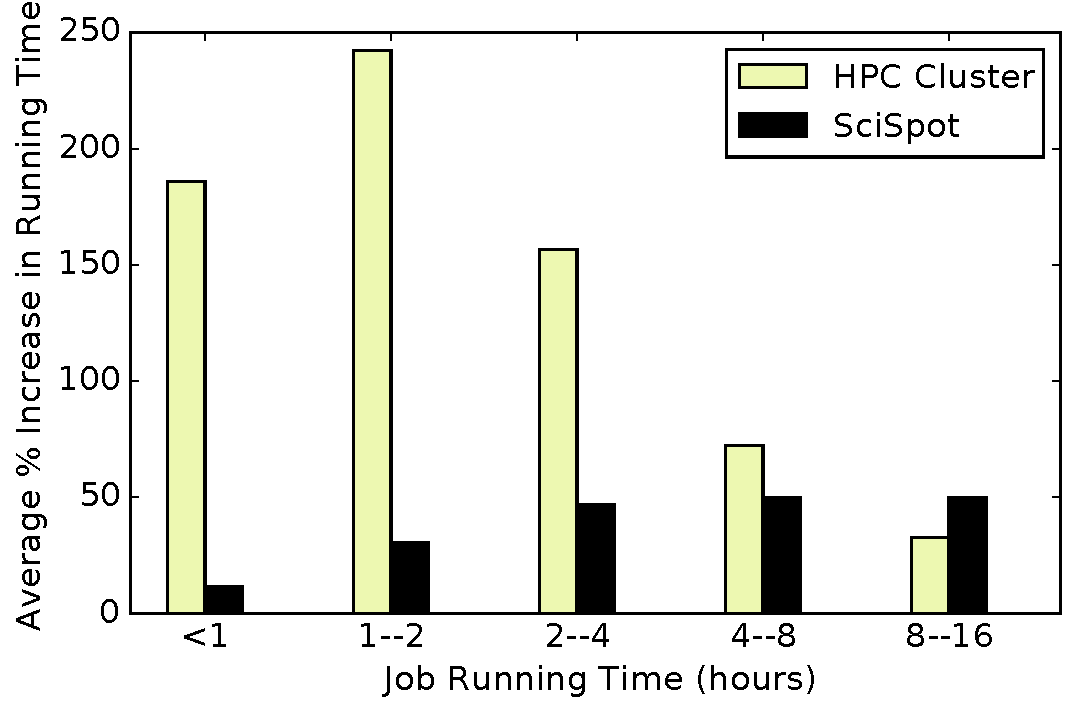
\includegraphics[width=0.4\textwidth]{../graphs/hpc-vs-scispot.pdf}
      \vspace*{\myfigspace}
  \caption{Increase in running time due to waiting/queuing on HPC clusters is significantly higher than the recomputation time for \sysname, especially for shorter jobs. }
  \label{fig:hpc-vs-scispot}
  \vspace*{\myfigspace}
\end{figure}


We define the overhead as the increase in running time which is equal to the turnaround time (i.e., the time between the job submission and successful completion) divided by the base job running time (with no waiting or premptions). 
%In HPC clusters, the overhead is the waiting time for resources, and in \sysname the overhead is the recomputation time due to preemptions.
Figure~\ref{fig:hpc-vs-scispot} compares the overhead (as percentage increase in running time) of \sysname and HPC clusters  for jobs of different lengths. We see that the average performance overhead due to waiting can be significant in the case of HPC clusters, and the job submission latency and queuing time dominate for smaller jobs, increasing their total turnaround time by more $2.5\times$.
This waiting is amortized in the case of longer running jobs, and the overhead drops off for longer jobs, to around 30\%.

On the other hand, \sysname's performance overhead is significantly smaller for jobs of up to 8 hours in length.
For longer jobs, the limited lifetime of Google Preemptible VMs (24 hours) begins to significantly increase the preemption probability and expected recomputation time.
We emphasize that these are \emph{individual} job lengths, and not the running time of entire bag of jobs.
We note that these large single jobs are rare, and for smaller jobs (within a much larger bag), both the preemption probability and recomputation overhead is much smaller. \vj{make more quantitative}

\noindent \emph{ \textbf{Result:} While preemptions can increase running times due to recomputation, this increase is small, and is between 20 to 400\% lower compared to the waiting times associated as overhead in conventional HPC clusters. }

\subsubsection{Comparison with HPC Performance}
The performance of scientific computing applications has been extensively compared on HPC and cloud setups~\cite{iosup_performance_2011, zhai_cloud_2011, marathe2013comparative, galante_analysis_2016, benedictis_cloud-aware_2014}. 
For completeness, we show the running times on the Big Red II supercomputing cluster in Table~\ref{tab:bigred2}, with 16 CPU nodes used throughout, and we see that our representative applications \emph{do not} face a penalty when deployed on the cloud. 

% This is confinement/shapes comparison against Big Red II
\begin{table}[]
  \begin{tabular}{|l|l|r|r|}
    \hline
    \# Application & Nodes & Big Red II & \sysname \\
    \hline
  	Nanoconfinement	&	1	&	2370	& 1546	\\
    Nanoconfinement	&	4	&	1140	&	851	\\
    \hline
  	Shapes	&	1	&	2649	& 1194	\\
    Shapes	&	4	&	1209	&	548	\\
    \hline
\end{tabular}
\caption{Running times (in seconds) of different applications on the Big Red II HPC cluster vs \sysname.}
\label{tab:bigred2}
  \vspace*{\myfigspace}
\end{table}




%%%%%%%%%%%%%%%%%%%%%%%%%%%%%%%%%%%%%%%%%%%%%%%%%%%%%%%%%%%%%%%%%%%%%%%%%%%%%%%%

\subsection{SciSpot Scaling}
We now turn our attention to \sysname's scaling properties. We are primarily interested in observing the behavior of running bags of jobs of different applications with different resource requirements.
In all cases unless otherwise stated, we run bags of 36 jobs, and impose that 90\% of all jobs complete (thus we target a completion of 32 jobs).
The jobs in the bags are for exploring the different parameters (i.e., doing a parameter sweep), using \sysname's automated parameter sweeping functionality described in Section~\ref{sec:impl}. For reference, the distribution of running times for the different applications is shown in Figure~\ref{fig:job-run-cdf}. 
In the rest of this section, we evaluate \sysname when the size of the cluster, the number of preemptions, and the number of jobs in the bag are increased.

\begin{figure}
  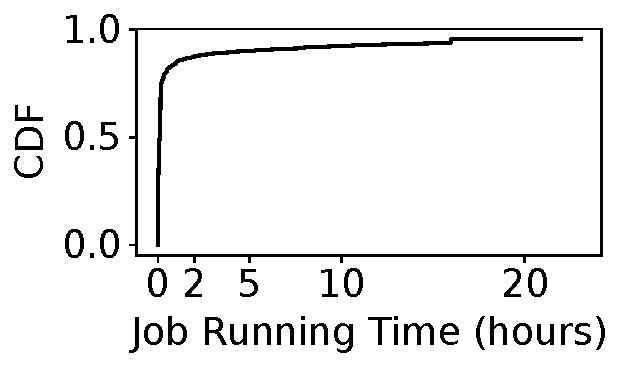
\includegraphics[width=0.2\textwidth]{../graphs/job-run-cdf.pdf}
  \vspace*{\myfigspace}
  \caption{Most HPC jobs are less than 2 hours.}
  \label{fig:job-run-cdf}
    \vspace*{\myfigspace}
\end{figure}

%%%%%%%%%%%%%%%%%%%%%%%%%%%%%%%%%%%%%%%%%%%%%%%%%%
%\vspace*{\subsecspace}
\subsubsection{Increasing Cluster Size} 

\begin{figure}
  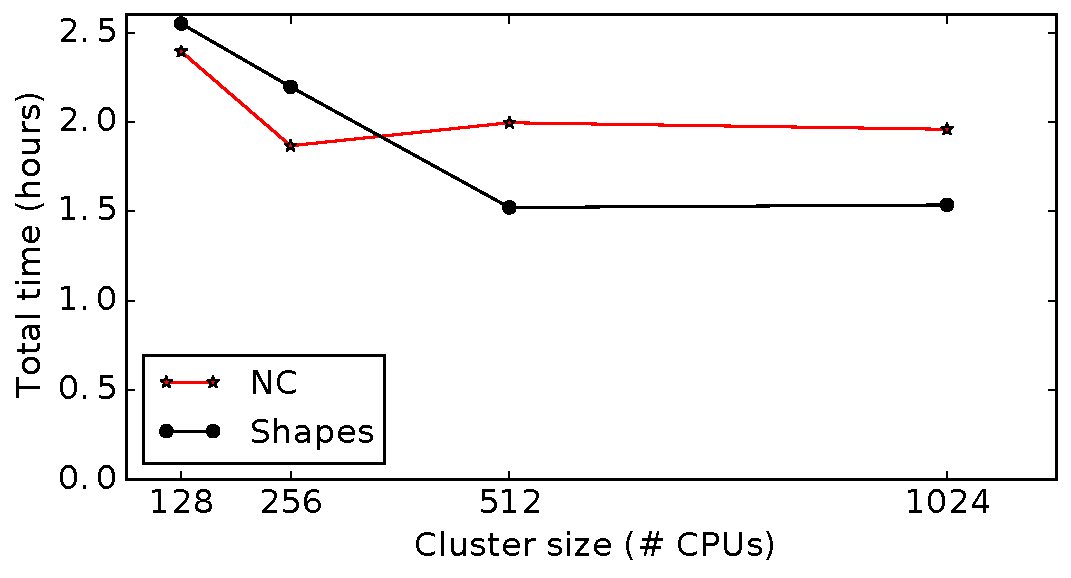
\includegraphics[width=0.4\textwidth]{../graphs/vm-per-job-scaling.pdf}
      \vspace*{\myfigspace}
  \caption{Bag of jobs running times exhibits classic parallel scaling behavior---performance improves until reaching a saturation point.}
  \label{fig:vm-per-job-scaling}
    \vspace*{\myfigspace}
\end{figure}

It is common to deploy scientific computing applications on large clusters, and we evaluate \sysname on different cluster sizes in Figure~\ref{fig:vm-per-job-scaling}.
The figure shows the total running time of the bag of jobs for the Nanoconfinement and Shapes applications as the total number of VMs (and hence total number of CPUs) increases.
For this experiment, we used \texttt{n1-highcpu-32} VMs with 32 CPUs each, and we ran four jobs in parallel on the entire cluster. 
We see classic scaling behavior: both applications can scale to a higher number of VMs up to a point, after which communication overhead starts to dominate, and the performance saturates and we see no reduction in running time. 


\begin{figure}
  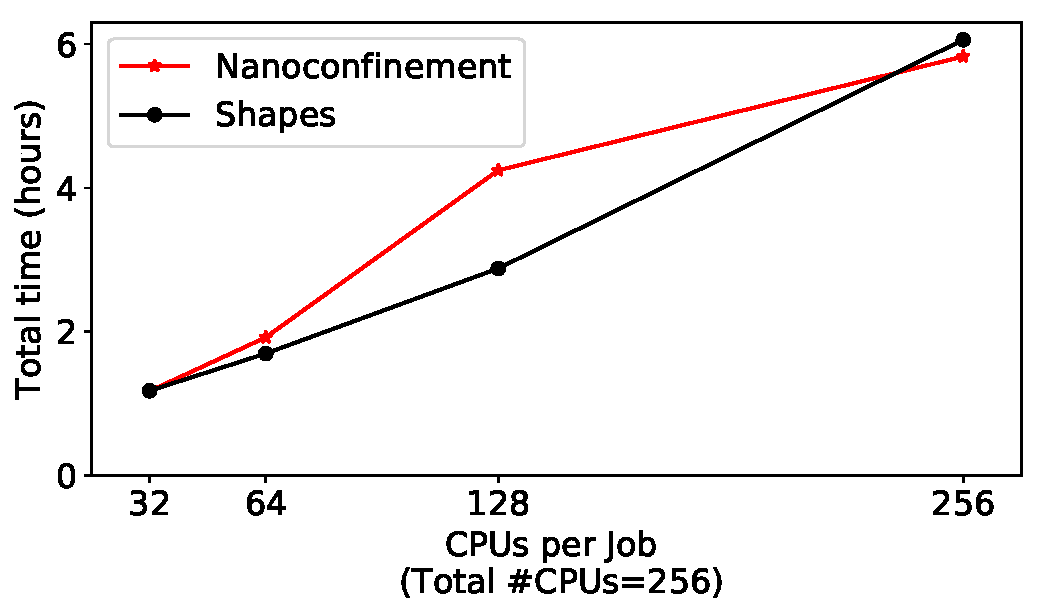
\includegraphics[width=0.2\textwidth]{../graphs/par-scaling.pdf}
      \vspace*{\myfigspace}
  \caption{\sysname can alleviate poor scaling by running more jobs in parallel and thus decreasing the intra-job parallelism (and hence number of CPUs per job, as shown in the figure).}
  \label{fig:par-scaling}
    \vspace*{\myfigspace}
\end{figure}


We note that \sysname provides the option to alleviate the parallel scaling bottleneck, by increasing the number of parallel jobs.
That is, for a given fixed cluster size, it can run more jobs in parallel, by reducing the total resources allocated and hence the parallelism 
of an individual job. 
The effect of changing the number of parallel jobs is shown in Figure~\ref{fig:par-scaling}, which shows the running time of an entire bag of jobs when the total cluster size is fixed (256 CPUs), but the number of parallel jobs and hence the number of CPUs per job changes.
We see that a \emph{smaller} number of CPUs per job limits the communication overhead, and thus reduces the total running time of the bag.
For both the NC and Shapes application, we see up to $6\times$ reduction in the total bag running time when more number of jobs are launched in parallel and a smaller number of CPUs per job are used. 


%%%%%%%%%%%%%%%%%%%%%%%%%%%%%%%%%%%%%%%%%%%%%%%%%%
\subsubsection{Increasing Bag Size}

We now evaluate \sysname's behavior when running larger bags of jobs.
Table~\ref{tab:100-jobs} shows the total running time of bags of 32 and 100 jobs.
Since \sysname reuses VMs when running jobs from a bag, it is able to take advantage of the relatively low preemption rates of VMs once they pass the first phase of early failures (Figure~\ref{fig:cdf}), and thus minimizes the number of preemptions as well as job failures. 
This makes \sysname particularly suitable for running the large bags of jobs that are required when using machine learning techniques for HPC workloads, an emerging research area in many science and engineering disciplines~\cite{ml.atomic2017,melko2017,sam2017,fu2017,long2015machine,ferguson2017machine,ward2018matminer,jcs1,jcs2,fox2019learning}, since the training and testing data needed for statistical machine learning can be generated through \sysname's bag of jobs execution model. 


%32_2_4 
\begin{table}
  \begin{tabular}{|c|r|r|r|}
    \hline
    Workload & Jobs & Time (Hours) & \# Preemptions \\
    \hline
    NC & 32  & 1.87 & 0 \\
    NC & 100  & 6.08 & 1 \\
    \hline
    Shapes & 32 & 1.47 & 0 \\
    Shapes & 100 & 4.49 & 5  \\  
    \hline
  \end{tabular}
  \caption{Running times and number of preemptions for bags of different sizes. }
  \label{tab:100-jobs}
  \vspace*{\myfigspace}
\end{table}




%%%%%%%%%%%%%%%%%%%%%%%%%%%%%%%%%%%%%%%%%%%%%%%%%%
\subsubsection{Increasing Preemptions}

By reusing VMs across a bag of jobs and taking advantage of the low preemption rates during the middle of the 24 hour life of the preemptible VMs, the \emph{expected} job failure rates and recomputation times are fairly small with \sysname (as shown in Figures~\ref{fig:runtimes-bar},~\ref{fig:hpc-vs-scispot}).
However, preemption rates can increase when the cloud operator sees high demand for resources.
Figure~\ref{fig:fails-time} shows the running time of the bag of 32 Nanoconfinement jobs on a cluster of 4 \texttt{n1-highcpu-32} VMs, when different number of VMs are preempted. 

We see that even with a high number of preemptions, the running time only increases by 50\%. 
We note that a higher than expected preemption rate (as shown in the figure) is rare, and happens with a vanishingly small likelihood. 
This shows that \sysname is robust and can provide acceptable performance even under extreme, adverse conditions. 

\begin{figure}[t]
  \centering 
  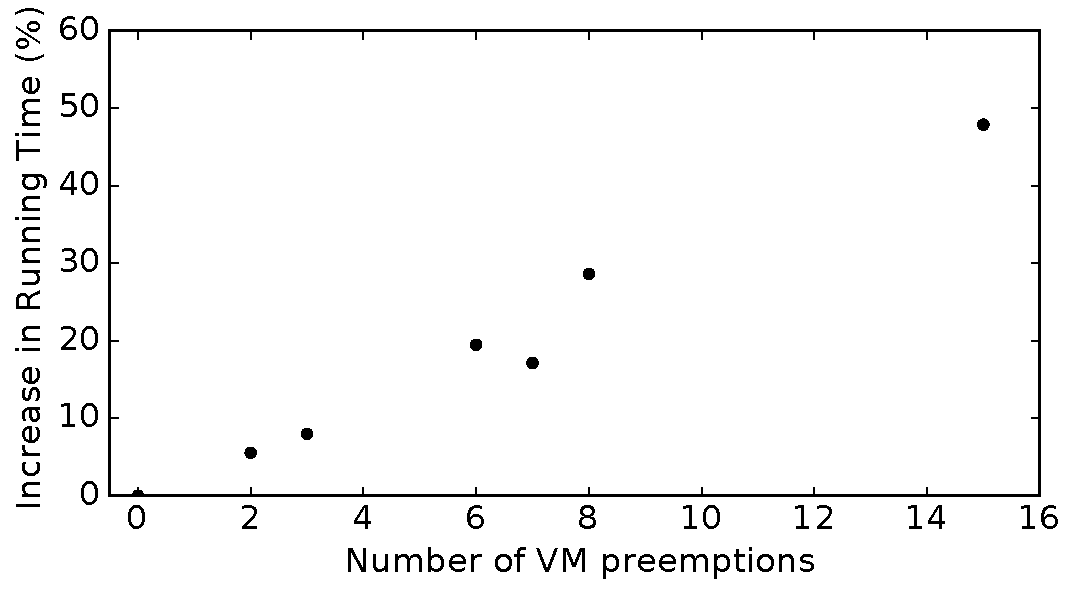
\includegraphics[width=0.4\textwidth]{../graphs/confin-fails-vs-time-relative.pdf}
      \vspace*{\myfigspace}
  \caption{The increase in running time due to preemptions is under 50\%, even when the number of preemptions is high.}
  \label{fig:fails-time}
\end{figure}


%Summary of results? 

%%%%%%%%%%%%%%%%%%%%%%%%%%%%%%%%%%%%%%%%%%%%%%%%%%


% \begin{figure}
%   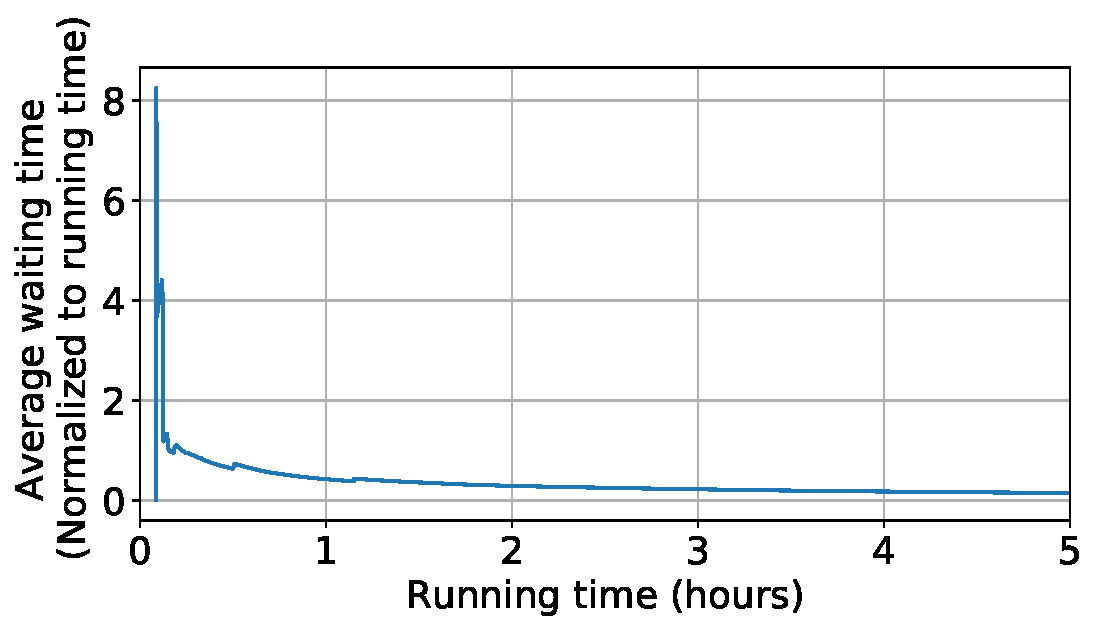
\includegraphics[width=0.4\textwidth]{../data/waiting_cumul.pdf}
%   \caption{The average waiting time (normalized to running time) of jobs of different length.}
%   \label{fig:hpc-wait-cdf}
% \end{figure}



%%% Local Variables:
%%% mode: latex
%%% TeX-master: "paper"
%%% End:


\vspace*{\subsecspace}
\section{Related Work}
\label{sec:related}


\sysname builds upon a large body of prior work on running scientific computing applications on the cloud, and the various facets of transient cloud computing.  

\vspace*{\subsecspace}
\subsection{Cloud Computing For Science}
Running scientific applications on the cloud introduces many tradeoffs compared to conventional HPC clusters, along the dimensions of performance, cost, scalability, convenience, and reproducability.
These tradeoffs are explored in~\cite{iosup_performance_2011, zhai_cloud_2011, marathe2013comparative, galante_analysis_2016, benedictis_cloud-aware_2014}.
In general, clouds can provide increased elasticity, lower waiting times, and more choices in resource allocation that can be tailored to the application.
The cloud resource model is also present in platforms like nanoHUB~\cite{nanohub}, that provide easy execution and dissemination of nanotechnology simulation applications.
%such as Ref.~\cite{kadupitiya2017}.
Outside of the bags of jobs execution model, price optimizations for scientific workflows in the cloud is discussed in~\cite{gari_learning_2019}. 
While bags of tasks~\cite{varshney_autobot_2019} are often used for parallel applications, \sysname is the first to use the bags of \emph{jobs} abstraction for efficient and effective use of transient servers. 

%\subsubsection{Bags of Jobs}
\vspace*{\subsecspace}
\subsection{Transient Cloud Computing}

%The low cost of transient cloud servers has made them very appealing, inspite of their preemptible nature, and their efficient and effective use has been a significant amount of research~\cite{prateek-thesis}. 
The challenges posed by Amazon EC2 spot instances, the first transient cloud servers, have received significant attention from both academia  and industry~\cite{spotinst}. 
Since spot instances are significantly cheaper than the equivalent on-demand servers, they are attractive for running preemption and delay tolerant batch jobs~\cite{spoton, jain14demand, yi2010reducing, conductor, liu-spot, spot-run, dubois2016optispot}.
A crucial component of EC2 spot instances is their dynamic auction-based pricing, and choosing the ``right'' bid price to minimize cost and performance degradation is the focus of much of the past work on transient computing~\cite{bidding4,mihailescu2012impact,bidding7,bidding1,bidding8,bidding3,bidding6,bid-cloud,bidding5,wolski_probabilistic_2017, guo_bidding_2015}.
However, as explained in Section~\ref{subsec:need-for-empirical}, it remains to be seen how Amazon's recent change~\cite{bid-change} in the preemption model of spot instances affects prior work.


On the other hand, the effective use of transient resources provided by other cloud providers such as Google, Microsoft, Packet, and Alibaba largely remains unexplored. 
Ours is the first work that studies the preemption characteristics and addresses the challenges involved in running large-scale applications on the Google Preemptible VMs, and provides insights on the unique preemption dynamics, as explained in Section~\ref{sec:preemption-dynamics}.

\vspace*{\subsecspace}
\subsubsection{Preemption Mitigation}
Effective use of transient servers usually entails the use of fault-tolerance techniques such as checkpointing~\cite{flint}, migration~\cite{spotcheck}, and replication.
In the context of HPC workloads,~\cite{marathe2014exploiting,gong_monetary_2015,xiang_spotmpi:_2011} develop checkpointing and bidding strategies for MPI applications running on EC2 spot instances, based on older spot pricing models. 
%, which are inherently memoryless and not applicable in our case. 
Periodic checkpointing~\cite{dongarra_fault_nodate} is not appropriate in our case because preemptions are not memoryless. 

By treating bags of jobs as an execution unit, allowing some jobs to fail, and using insights from preemption models, we show that it is possible to reduce the recomputation times to acceptable levels even without the  use of periodic  checkpointing that imposes additional deployment and performance overheads. 
%The first step towards mitigating preemptions is understanding their characteristics. 
Our preemption model for Google preemptible VMs developed in Section~\ref{sec:preemption-dynamics} provides a novel characterization of bathtub shaped failure rates not captured by the classic Weibull distribution, and is distinct from prior efforts~\cite{mudholkar1993exponentiated, crevecoeur1993model}. 

%extends the classic Weibull-distribution based bathtub models~\cite{mudholkar1993exponentiated, crevecoeur1993model} by introducing exponential reclamation near the deadline and additional paramters that capture and explain the preemption dynamics. 

\vspace*{\subsecspace}
\subsubsection{Server Selection}

Optimized server selection is an important problem in cloud computing, and especially for transient servers because of the cost-performance-preemption tradeoff involved. 
Similar to \sysname, SpotOn~\cite{spoton} is also a batch computing service that selects servers based on job characteristics and failure rates of different EC2 spot VMs. However, it is restricted to individual, single-VM batch jobs, and its design is tied to EC2 spot instances.
The state of the art transient server selection involves the use of multiple types of VMs~\cite{exosphere}, and selecting a heterogeneous cluster can reduce the likelihood of mass concurrent preemptions.
However, since scientific computing applications are mostly synchronous, even a single failure affects the entire job, and heterogeneous clusters are not required, and are in fact, detrimental~\cite{exosphere}. 
Server selection is important even outside of preemptible VMs---developing bayesian optimization and application performance model based search for the ``best'' cloud VM is an active research area~\cite{alipourfard_cherrypick, yadwadkar_selecting_2017}, but these techniques do not  account  for preemptions. 

\begin{figure}[t]
  \centering 
       \vspace*{\myfigspace} 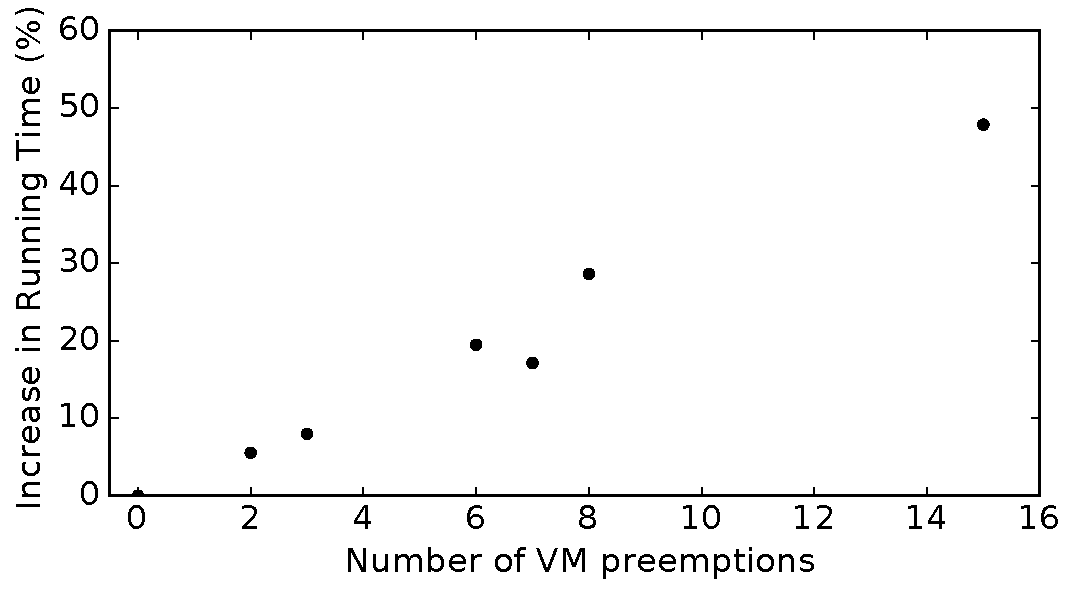
\includegraphics[width=0.22\textwidth]{../graphs/confin-fails-vs-time-relative.pdf}
      \vspace*{\myfigspace}
  \caption{The increase in running time due to preemptions is under 50\%, even when the number of preemptions is high.}
  \label{fig:fails-time}
        \vspace*{\myfigspace}
\end{figure}




\vspace*{\subsecspace}
%Parameter sweep aka bags of jobs ~\cite{casanova_heuristics_2000}

%But nothing for bags of jobs themselves.. 


% \subsubsection{Fault-tolerance}

% All the past work was on EC2 spot market with gang failures and independent markets~\cite{marathe2014exploiting, gong_monetary_2015}.
% However this assumption has now changed, and failures can happen anytime.
% Our failure model is more general, and applies to both cases.



% \cite{dongarra_fault_nodate} has a discussion of checkpointing frequency which is comprehensive. Replication is another way~\cite{walters_replication-based_2009}

% Non periodic checkpointing~\cite{bougeret_checkpointing_2011}


% \subsubsection{Failure Modeling}



% Crevecour etc. 



% \subsubsection{Server Selection}
% Exploring a large configuration space using bayesian optimization methods in CherryPick~\cite{alipourfard_cherrypick} and Metis~\cite{li2018metis}.

% Can also use Latin Hypercube sampling for parameter exploration?




%%% Local Variables:
%%% mode: latex
%%% TeX-master: "paper"
%%% End:


%% 10 pages plus references 

{
\bibliographystyle{acm}
\interlinepenalty=10000 %%%%For fixing url-related errors only 
\bibliography{scicloud}
}


\end{document}


%%% Local Variables:
%%% mode: latex
%%% TeX-master: t
%%% End:
